\documentclass[10pt]{beamer}

\usepackage{tikz, hyperref, alltt}
\usetikzlibrary{positioning,shapes,shadows,arrows}
\tikzstyle{abstract}=[rectangle, rounded corners, draw=black, anchor=north, fill=blue!10, text centered, minimum height={height("Gp")+2pt}, minimum width=3cm, font=\footnotesize]

\definecolor{links}{HTML}{0000CC}
\hypersetup{colorlinks,linkcolor=,urlcolor=links}

\mode<handout>
{
  \usepackage{pgfpages}
  \pgfpagesuselayout{4 on 1}[a4paper,border shrink=3mm,landscape]
  \usetheme{CambridgeUS}
  \usecolortheme{lily}
}

\mode<beamer>
{
  \usetheme{CambridgeUS}
}

\AtBeginSection[]
{
  \begin{frame}
    \frametitle{Outline}
    \tableofcontents[currentsection]
  \end{frame}
}

\setbeamerfont{frametitle}{family=\rmfamily,series=\bfseries,size={\fontsize{10}{10}}}
\setbeamertemplate{frametitle continuation}[from second]

\title{Dynare Time Series \& Reporting}
\author[Houtan Bastani]{Houtan Bastani\newline\href{mailto:houtan@dynare.org}{houtan@dynare.org}}
\institute{CEPREMAP}
\date{13 June 2014}

\newcommand{\myitem}{\item[$\bullet$]}

\begin{document}

\begin{frame}
  \titlepage
\end{frame}

\begin{frame}[t]
  \frametitle{Outline}
  \tableofcontents
\end{frame}

%
% DATES
%
\section{Time Series}

\subsection{Overview}
\begin{frame}[fragile,t]
  \frametitle{Overview}
  \begin{itemize}
  \myitem Provide support for time series (\texttt{dseries})
    \begin{itemize}
    \myitem Based on an implementation for handling dates (\texttt{dates})
    \end{itemize}
  \myitem Beta version in Dynare 4.4. Mature version ready in Dynare 4.5
  \myitem Currently only used for reporting, though use will increase with time
    (\textit{e.g.,} to be included in new estimation code)
  \myitem Compatible with all setups that are supported by Dynare
    \begin{itemize}
    \myitem Windows, Mac OS X, Linux
    \myitem Matlab 7.5 (R2007b) or later, Octave
    \end{itemize}
  \myitem NB: More complete information is included in the Dynare manual
  \end{itemize}
\end{frame}


\subsection{A Programming Note}
\begin{frame}[fragile,t]
  \frametitle{A Programming Note (1/2)}
  \begin{itemize}
  \myitem Time series and dates are implemented as Matlab/Octave classes
  \myitem Inplace modification of instantiated objects not supported. Let me explain \dots
    \begin{itemize}
      \myitem A class is a template for defining objects, defining their member
      variables and methods.
      \begin{itemize}
        \myitem \textit{e.g.,} The \texttt{dates} class defines 3 member
        variables--\texttt{ndat}, \texttt{freq}, and \texttt{time}--and many
        methods (analogous to functions)
      \end{itemize}
      \myitem An object is an instance of a specific class. For exemplary
      purposes, imagine an object \texttt{X}, which is an instantiation of the
      class ``Integer''. The object has value \texttt{1}:
\begin{verbatim}
>> X

X =

     1
\end{verbatim}
    \myitem You can call any method defined for the integer class on integer
    object \texttt{X}. Imagine such a method is called
    \texttt{multiplyByTwo()}.
    \myitem In most object-oriented
    languages, writing \texttt{X.multiplyByTwo();} will change the value
    contained in \texttt{X} to \texttt{2/2}
    \end{itemize}
  \end{itemize}
\end{frame}


\begin{frame}[fragile,t]
  \frametitle{A Programming Note (2)}
  \begin{itemize}
    \item[] \begin{itemize}
  \myitem But! For Matlab/Octave's implementation of classes this is not the
    case as it does not support inplace modification
\begin{verbatim}
>> X.multiplyByTwo()

ans =

     2

>> X

X =

     1
\end{verbatim}
  \end{itemize}
  \end{itemize}
\end{frame}

\begin{frame}[fragile,t]
  \frametitle{A Programming Note (concluded)}
  \begin{itemize}
    \item[] \begin{itemize}
    \myitem To get the desired change, you must overwrite \texttt{X}
\begin{verbatim}
>> X=X.multiplyByTwo()

X =

     2
\end{verbatim}
\myitem Keep this in mind when using Dynare dates, time series, and reporting
  \end{itemize}
  \end{itemize}
\end{frame}


\subsection{Syntax}
\begin{frame}[fragile,t]
  \frametitle{Syntax}
  \begin{itemize}
  \myitem Two components of a time series:
    \begin{itemize}
    \myitem A time component. In Dynare: \texttt{dates}
    \myitem A data component mapped to time. In Dynare: \texttt{dseries}
    \end{itemize}
  \end{itemize}
\end{frame}

\subsubsection{\texttt{dates} Syntax}
\begin{frame}[fragile,t]
  \frametitle{\texttt{dates} Syntax}
  \begin{itemize}
    \myitem The \texttt{dates} command creates an object that represents at least one date at a given frequency
    \myitem A \texttt{dates} object contains 3 members (fields):
    \begin{itemize}
      \myitem{\textbf{\texttt{freq}}}: 1 (Annual), 4 (Quarterly), 12 (Monthly), 52 (Weekly)
      \myitem{\textbf{\texttt{ndat}}}: The number of dates
      \myitem{\textbf{\texttt{time}}}: An \texttt{ndat$\times$2} matrix; the 1\textsuperscript{st} col is the year and the 2\textsuperscript{nd} col is the period
    \end{itemize}
    \myitem \texttt{dseries} members cannot be modified. Thus, this is not allowed:
\begin{alltt}
  >> dd.freq = 12;
\end{alltt}
  \end{itemize}
\end{frame}


\begin{frame}[fragile,t]
  \frametitle{Creating a new \texttt{dates} object in Matlab/Octave}
  \begin{itemize}
    \myitem{A single date}
\begin{alltt}
  >> t = dates(`1999y');
\end{alltt}
    \myitem{Multiple dates}
\begin{alltt}
  >> t = dates(`1999q1', `2020q2', `-190q3');
\end{alltt}
Notice that noncontiguous and negative dates are possible
    \myitem{A date range}
\begin{alltt}
  >> dr = dates(`1999y'):dates(`2020y');
\end{alltt}
    \myitem Can also create \texttt{dates} programatically
\begin{alltt}
  >> t = dates(4, [1990; 1990; 1978], [1; 2; 3])
  t = <dates: 1990Q1, 1990Q2, 1978Q3>
\end{alltt}
    \myitem Can specify an empty \texttt{dates}\dots
\begin{alltt}
  >> qq = dates(`Q');
  >> qq = dates(4);
\end{alltt}
    \myitem \dots and use it to instantiate new \texttt{dates}
\begin{alltt}
  >> t = qq(1990, 1);
  t = <dates: 1990Q1>
\end{alltt}
\begin{alltt}
  >> t = qq([1990; 1990; 1978], [1; 2; 3])
  t = <dates: 1990Q1, 1990Q2, 1978Q3>
\end{alltt}
  \end{itemize}
\end{frame}



\begin{frame}[fragile,t]
  \frametitle{Creating a new \texttt{dates} object in a \texttt{.mod} file}
  \begin{itemize}
    \myitem The preprocessor allows for syntax simplification when
    \texttt{dates} are in \texttt{.mod} files
    \myitem{A single date} \texttt{t = 1999y;}
\begin{alltt}
  \(\Rightarrow\) t = dates(`1999y');
\end{alltt}
    \myitem{Multiple dates} \texttt{t = [1999q1 2020q2 1960q3];}
\begin{alltt}
  \(\Rightarrow\) t = [dates(`1999q1') dates(`2020q2') dates(`1960q3')];
\end{alltt}
    \myitem{A date range} \texttt{dr = 1999y:2020y;}
\begin{alltt}
  \(\Rightarrow\) dr = dates(`1999y'):dates(`2020y');
\end{alltt}
    \myitem NB: This can cause problems when dates are included in strings. \textit{e.g.,}
\begin{alltt}
  disp(`In 1999q1, ...')
\end{alltt}
would be transformed into
\begin{alltt}
  disp(`In dates(`1999q1'), ...')
\end{alltt}
      \myitem To fix this, simply escape any date that you don't want transformed by the preprocessor with a `\texttt{\$}'
\begin{alltt}
  disp(`In $1999q1, ...')
\end{alltt}

  \end{itemize}
\end{frame}


\begin{frame}[fragile,t]
  \frametitle{Collections and Ranges of \texttt{dates} in a \texttt{.mod} file}
  \begin{itemize}
    \myitem A collection of \texttt{dates}
    \begin{alltt}
  a = 1990Q1; b = 1957Q1; c = -52Q1;
  d = [a b c];
  \(\Rightarrow\) d = <dates: 1990Q1, 1957Q1, -52Q1>
    \end{alltt}
    \myitem A Range of \texttt{dates}
    \begin{alltt}
  a = 1990Q3:1991Q2
  \(\Rightarrow\) a = <dates: 1990Q3, 1990Q4, 1991Q1, 1991Q2>
    \end{alltt}
    \myitem A set of regularly-spaced \texttt{dates}
    \begin{alltt}
  a = 1990Q3:2:1991Q2
  \(\Rightarrow\) a = <dates: 1990Q3, 1991Q1, 1991Q3>
    \end{alltt}
  \end{itemize}
\end{frame}


\begin{frame}[fragile,t]
  \frametitle{Comparing \texttt{dates}}
  \begin{itemize}
    \myitem The following comparison operators are supported: $==$, $\backsim=$, $<$, $\leq$, $>$, and $\geq$
    \myitem Compared objects must have the same frequency
    \myitem Compared objects must have the same number of elements (except for singletons)
    \myitem Returns the result of an element-wise comparison
    \myitem Let \texttt{a=[1999W1 2020W3]}, \texttt{b=1999W1}, and \texttt{c=[1888w1 2020w3]}. Then
    \begin{alltt}
  >> a == b              >> a > b              >> c < a

  ans =                  ans =                 ans =

       1                      0                     1
       0                      1                     0
    \end{alltt}
  \end{itemize}
\end{frame}



\begin{frame}[fragile,t]
  \frametitle{Arithmetic Operations on \texttt{dates}}
  \begin{itemize}
    \myitem The unary \texttt{+} and \texttt{-} operators
    \begin{alltt}
  >> a = dates(`1999q4');
  >> +a \(\Rightarrow\) ans = 2000q1
  >> -a \(\Rightarrow\) ans = 1999q3
  >> ++-+a \(\Rightarrow\) ans = 2000q2
    \end{alltt}
    \myitem The binary \texttt{+} and \texttt{-} operators
    \begin{itemize}
      \myitem Objects must have the same frequency
      \myitem Objects must have the same number of elements (except for singletons)
      \myitem \texttt{1999q4 + 2} $\Rightarrow$ \texttt{ans = 2000q2}
      \myitem \texttt{1999w4 + 2} $\Rightarrow$ \texttt{ans = 1999w6}
      \myitem \texttt{1999m4 - 2} $\Rightarrow$ \texttt{ans = 1999m2}
      \myitem \texttt{1999m4 - 1999m2} $\Rightarrow$ \texttt{ans = 2}
      \myitem \texttt{1999m4 + 1999m2} $\Rightarrow$ \texttt{ans = <dates: 1999M4, 1999M2>}
    \end{itemize}
    \myitem The binary \texttt{*} operator
    \begin{alltt}
  >> a*3
  ans = <dates: 1999Q4, 1999Q4, 1999Q4>
    \end{alltt}
  \end{itemize}
\end{frame}



\begin{frame}[fragile,t]
  \frametitle{Set Operations on \texttt{dates}}
  \begin{itemize}
    \myitem Let \texttt{a = [1990Q1:1991Q1 1990Q1]; b = [1990Q3:1991Q3];}
    \myitem \texttt{intersect}: returns the intersection of the arguments
    \begin{alltt}
  >> intersect(a, b)
  ans = <dates: 1990Q3, 1990Q4, 1991Q1>
    \end{alltt}
    \myitem \texttt{setdiff}: returns dates present in first arg but not in second
    \begin{alltt}
  >> setdiff(a, b)
  ans = <dates: 1900Y>
    \end{alltt}
    \myitem \texttt{union}: returns the union of two sets (repititions removed)
    \begin{alltt}
  union(a, b)
  ans = <dates: 1990Q1, 1990Q2,  ..., 1991Q2, 1991Q3>
    \end{alltt}
    \myitem \texttt{unique()}: removes repititions from set (keeps last unique value)
    \begin{alltt}
  >> a.unique()
  ans = <dates: 1990Q2, 1990Q3, 1990Q4, 1991Q1, 1990Q1>
    \end{alltt}
  \end{itemize}
\end{frame}



\begin{frame}[fragile,t]
  \frametitle{Misc \texttt{dates} operations}
  \begin{itemize}
    \myitem Can index a \texttt{dates} object.
    \begin{alltt}
  >> a = dates(`2000y'):dates(`2009y');
  >> a(1)
  ans = <dates: 2000Y>
  >> a(1:3)
  ans = <dates: 2000Y, 2001Y, 2002Y>
  >> a([1,4,5])
  ans = <dates: 2000Y, 2003Y, 2004Y>
    \end{alltt}
    \myitem{\textbf{\texttt{pop()}}}: Remove last element
    \begin{alltt}
  >> a.pop()
  ans = <dates: 2000Y, 2001Y,  ..., 2007Y, 2008Y>
    \end{alltt}
    \myitem{\textbf{\texttt{char()}}}: Return string representation
    \begin{alltt}
  >> a(1).char()
  ans = 2000Y
    \end{alltt}
    \myitem More in the Dynare manual
  \end{itemize}
\end{frame}


%
% DSERIES
%
\subsubsection{\texttt{dseries} Syntax}
\begin{frame}[fragile,t]
  \frametitle{\texttt{dseries} Syntax}
  \begin{itemize}
    \myitem A \texttt{dseries} is composed of one or more individual time series
    \myitem All time series in a \texttt{dseries} must have the same frequency
    \myitem A \texttt{dseries} runs from the earliest date to the latest date,
    with \texttt{NaN}'s inserted to pad the shorter series
    \myitem A \texttt{dseries} object contains 3 members:
    \begin{itemize}
      \myitem{\textbf{\texttt{data}}}: The data points
      \myitem{\textbf{\texttt{dates}}}: The \texttt{dates} of the sample
      \myitem{\textbf{\texttt{name}}}: Names of the variables
      \myitem{\textbf{\texttt{nobs}}}: The number of observations
      \myitem{\textbf{\texttt{vobs}}}: The number of variables
      \myitem{\textbf{\texttt{tex}}}: \LaTeX\ names of the variables
    \end{itemize}
    \myitem \texttt{dseries} members cannot be modified
  \end{itemize}
\end{frame}


\begin{frame}[fragile,t]
  \frametitle{Creating a new \texttt{dseries} object (1/2)}
  Load data directly
  \begin{itemize}
    \myitem Syntax:
    \begin{alltt}
  ts = dseries(DATA, INITIAL_PERIOD, NAMES, TEX_NAMES)
    \end{alltt}
    \myitem \textit{e.g.,} 2 variables, `MyVar1' and `MyVar2', with
    3 annual observations starting in 1999:
\small{
    \begin{alltt}
  >> ts = dseries([1 2;3 4;5 6], `1999y', ...
                 \{`MyVar1', `MyVar2'\}, \{`MyVar\_1', 'MyVar\_2'\});

  ts is a dseries object:

        | MyVar1 | MyVar2
  1999Y | 1      | 2
  2000Y | 3      | 4
  2001Y | 5      | 6
    \end{alltt}}
  \end{itemize}
\end{frame}

\begin{frame}[fragile,t]
  \frametitle{Creating a new \texttt{dseries} object (2/2)}
  Load series from CSV/spreadsheet (\texttt{.csv, .xls}) or Matlab file (\texttt{.m, .mat})
  \begin{itemize}
    \myitem Syntax:
    \begin{alltt}
  >> ts = dseries(FILENAME);
    \end{alltt}
    \myitem File format (\texttt{.csv, .xls}): dates in first column (using the standard format:
    199Q1 for quarterly data, 1990Y for annual data, \dots) and (optional)
    variable names in the first row
    \myitem File format (\texttt{.m, .mat}): must define the variables \texttt{INIT\_\_},
    \texttt{NAMES\_\_}, and, optionally, \texttt{TEX\_\_}. More info in the
    manual. Data are vectors.
    \begin{alltt}
      INIT__ = `1999q1’;
      NAMES__ = \{`cons'\};
      cons = randn(100,1);
    \end{alltt}
  \end{itemize}
  Create an empty time series. Usefull for programatically creating a series.
  \begin{itemize}
    \myitem \texttt{ts=dseries();}
    \myitem \texttt{ts=dseries(dates(`1999y'));}
  \end{itemize}
\end{frame}



\begin{frame}[fragile,t]
  \frametitle{Creating subsamples from a \texttt{dseries}}
  \begin{itemize}
    \myitem Let \texttt{ts} be a \texttt{dseries} with $N$ variables and 5
    observations from \texttt{2000Y} to \texttt{2004Y}
    \myitem To obtain a subsample from \texttt{2001Y} to \texttt{2003Y}
    \begin{alltt}
  ts(2001Y:2003Y)
    \end{alltt}
    \myitem Can also use integer indices
    \begin{alltt}
  start = find(ts.dates==2001Y);
  ts(start:end);
    \end{alltt}
    \myitem NB: Integer indices cannot be used to extract a single observation
    because of lag/lead notation (see below)
  \end{itemize}
\end{frame}



\begin{frame}[fragile,t]
  \frametitle{Extracting variables from a \texttt{dseries}}
  \begin{itemize}
    \myitem Let
    \begin{alltt}
  >> ts = dseries(randn(5,6), `2000q1', ...
                 \{`GDP_US', `GDP_FR', `GDP_JA', ...
                  `CPI_US', `CPI_FR', `CPI_JA'\});
    \end{alltt}
    \myitem We can extract one variable using syntax like
    \begin{alltt}
  >> ts.GDP_US
    \end{alltt}
    \myitem To get all the \texttt{GDP} variables
    \begin{alltt}
  >> ts\{`GDP_US', `GDP_FR', `GDP_JA'\}
    \end{alltt}
    \myitem A shorter way to do the same thing
    \begin{alltt}
  >> ts\{`GDP_@US,FR,JA@'\}
    \end{alltt}
    \myitem To get \texttt{GDP} \& \texttt{CPI} (NB: max 2 implicit loops)
    \begin{alltt}
  >> ts\{`@GDP,CPI@_@US,FR,JA@'\}
    \end{alltt}
  \end{itemize}
\end{frame}


\begin{frame}[fragile,t]
  \frametitle{Applying methods to \texttt{dseries}}
  \begin{itemize}
    \myitem Suppose \texttt{ts} is as above. Then, to apply a method
    (\textit{e.g.,} \texttt{log()}) to \texttt{GDP}:
    \begin{alltt}
  ts\{`GDP_@US,FR,JA@'\}=ts\{`GDP_@US,FR,JA@'\}.log()
    \end{alltt}
    \myitem To apply a method to a subsample of all the variables:
    \begin{alltt}
  ts(2000Q2:2000Q4) = ts(2000Q2:2000Q4).log()
    \end{alltt}
    \myitem To apply a method to a subsample of some of the variables:
    \begin{alltt}
  ts(2000Q2:2000Q4)\{`GDP_@US,FR,JA@'\} = ...
    ts(2000Q2:2000Q4)\{`GDP_@US,FR,JA@'\}.log()
    \end{alltt}
  \end{itemize}
\end{frame}


\begin{frame}[fragile,t]
  \frametitle{Merging \texttt{dseries}}
  \begin{itemize}
    \myitem Suppose that \verb+ts+ and \verb+ds+ are two \texttt{dseries} objects
    with the same variables observed on different time ranges. These
    \texttt{dseries} objects can be merged using the following syntax:
\begin{verbatim}
    vs = [ts; ds];
\end{verbatim}
\myitem Suppose that \verb+ts+ and \verb+ds+ are two \texttt{dseries} objects
with different variables observed on the same or different time ranges. These
\texttt{dseries} objects can be merged using the following syntax:
\begin{verbatim}
    vs = [ts, ds];
\end{verbatim}
If \verb+ts+ and \verb+ds+ are not defined over the same time range,
the time range of \verb+vs+ will be the union of \verb+ts.dates+ and
\verb+ds.dates+, \verb+NaN+s will be added for the missing observations.
  \end{itemize}
\end{frame}


\begin{frame}[fragile,t]
  \frametitle{Arithmetic Operations on \texttt{dseries}}
  \begin{itemize}
    \myitem The binary operators \texttt{+}, \texttt{-}, \texttt{*},
    \texttt{/}, and \texttt{\string^} perform element-wise arithmetic operations on
    \texttt{dseries}
    \myitem They can be used with two \texttt{dseries} or one \texttt{dseries}
    and a real number
    \myitem Two \texttt{dseries} can have different date ranges. Non overlapping dates will be filled with \texttt{NaNs}
    \myitem Take addition for example
    \begin{itemize}
      \myitem Let
    \begin{alltt}
>> ts0 = dseries(ones(2,2)*2, `2000W1', \{`MyVar1', `MyVar2'\});
>> ts1 = dseries(ones(3,2)*3, `2000W2', \{`YrVar1', `YrVar2'\});
>> ds = ts0.MyVar1;
    \end{alltt}
    \myitem \texttt{ts0+3} will add \texttt{3} to every element in \texttt{ts0}
    \myitem \texttt{ts0+[3 4]} will add \texttt{3} to every element in \texttt{ts0.MyVar1} and \texttt{4} to every element in \texttt{ts0.MyVar2}
    \myitem \texttt{ts0+ts1} will add \texttt{ts0.MyVar1} to \texttt{ts1.YrVar1} and \texttt{ts0.MyVar2} to \texttt{ts1.YrVar2}. Only \texttt{2000W2} will contain the value \texttt{5} for both variables. All other points will contain \texttt{NaN}
    \myitem \texttt{ts0+ds} will add \texttt{ds} to \texttt{ts0.MyVar1} and \texttt{ts0.MyVar2}. All values will contain \texttt{4}
    \end{itemize}
  \end{itemize}
\end{frame}



\begin{frame}[fragile,t]
  \frametitle{Leads and Lags with \texttt{dseries} (1/2)}
  \begin{itemize}
    \myitem Let
    \begin{alltt}
  >> ts = dseries([1:4]');
    \end{alltt}
    \myitem Then
    \begin{alltt}
  >> ts.lead()                      >> ts.lag()

  ans is a dseries object:          ans is a dseries object:

     | lead(Variable_1,1)              | lag(Variable_1,1)
  1Y | 2                            1Y | NaN
  2Y | 3                            2Y | 1
  3Y | 4                            3Y | 2
  4Y | NaN                          4Y | 3
    \end{alltt}
  \end{itemize}
\end{frame}


\begin{frame}[fragile,t]
  \frametitle{Leads and Lags with \texttt{dseries} (2/2)}
  \begin{itemize}
    \myitem You can lead/lag a \texttt{dseries} by more than one period
    \begin{itemize}
      \myitem \texttt{ts.lead(k)} where $k\in\mathbb{Z}$
      \myitem \texttt{ts.lag(k)} where $k\in\mathbb{Z}$
    \end{itemize}
    \myitem A shorthand syntax is available as well
    \begin{itemize}
      \myitem Lead: \texttt{ts(k)} where $k\in\mathbb{Z}$
      \myitem Lag: \texttt{ts(-k)} where $k\in\mathbb{Z}$
    \end{itemize}
  \end{itemize}
\end{frame}




%
% REPORTING
%
\section{Reporting}
\subsection{Overview}
\begin{frame}[fragile,t]
  \frametitle{Overview}
  \begin{itemize}
  \myitem Beta version in Dynare 4.4. Mature version ready in Dynare 4.5
  \myitem Introduce reporting functionality to Dynare
      \begin{itemize}
      \myitem Input: \texttt{dseries}
      \myitem Output: \LaTeX\ report \& compiled \texttt{.pdf}
      \end{itemize}
    \myitem Graphs and Tables are modular
      \begin{itemize}
      \item[$\Rightarrow$] Can easily be included in another document
      \end{itemize}
    \myitem Graphs are produced in Ti$k$Z/PGFPlots (standard in a \TeX\ distribution)
      \begin{itemize}
      \myitem Scales well
      \myitem Formating follows that of enclosing document
      \end{itemize}
    \myitem Dynare provides a subset of the many Ti$k$Z options
      \begin{itemize}
      \myitem You can easily modify the Ti$k$Z graph if the option you want is not in Dynare
      \end{itemize}
    \myitem Works with Matlab \& Octave
    \myitem Works much faster than similar softawre
    \myitem NB: Must install a \LaTeX\ distribution to compile reports
      \begin{itemize}
      \myitem On Windows use MiKTeX: \url{http://miktex.org}
      \myitem On Mac OS X use MacTeX: \url{http://tug.org/mactex}
      \myitem On Linux use \TeX\ Live: available from your package manager
      \end{itemize}
  \end{itemize}
\end{frame}


\begin{frame}[fragile,t]
  \frametitle{How Reporting Works}
  \begin{itemize}
    \myitem Reports are created command by command
    \begin{itemize}
    \myitem Hence the order of commands matters
    \end{itemize}
  \myitem All reporting commands act on the previously added object until an object of greater or equal hierarchy is added (see next slide)
    \begin{itemize}
    \myitem \textit{e.g.,} Once you add a \texttt{Page} to your report with the \texttt{addPage()} command, every \texttt{Section} you add via the \texttt{addSection()} command will be placed on this page. Only when you add another \texttt{Page} will items go on a new page.
    \myitem This will become more clear with an example
    \end{itemize}
  \myitem Options to reporting commands are passed in option name/value pairs
    \begin{itemize}
    \myitem \textit{e.g.,} \texttt{addPage(`title', \{`Page Title', `Page Subtitle'\})}
    \end{itemize}
  \end{itemize}
\end{frame}


\begin{frame}[fragile,t]
  \frametitle{Reporting Class Hierarchy}
  \begin{itemize}
  \myitem Class names on the top half of the box, constructor names on the bottom
  \myitem Arrows represent what the new object can be added to
  \end{itemize}
  \begin{center}
    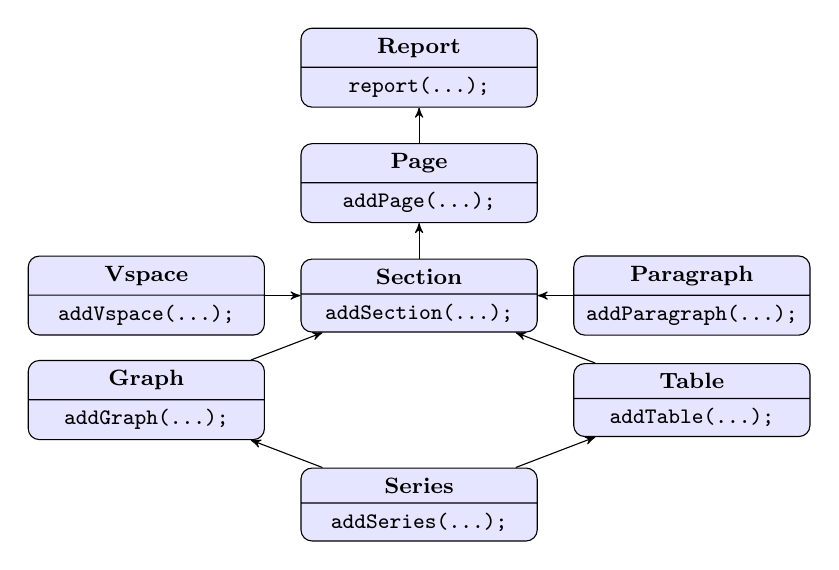
\begin{tikzpicture}[
        node distance = .45cm,
        auto,
        line/.style={->, >=stealth'},
      ]
      \node (Report) [abstract, rectangle split, rectangle split parts=2]
            {
              \textbf{Report}
              \nodepart{second}\texttt{report(...);}
            };
      \node (Page) [abstract, rectangle split, rectangle split parts=2, below=of Report]
            {
              \textbf{Page}
              \nodepart{second}\texttt{addPage(...);}
            };
      \node (Section) [abstract, rectangle split, rectangle split parts=2, below=of Page]
            {
              \textbf{Section}
              \nodepart{second}\texttt{addSection(...);}
            };
      \node (Paragraph) [abstract, rectangle split, rectangle split parts=2, right=of Section]
            {
              \textbf{Paragraph}
              \nodepart{second}\texttt{addParagraph(...);}
            };
      \node (Vspace) [abstract, rectangle split, rectangle split parts=2, left=of Section]
            {
              \textbf{Vspace}
              \nodepart{second}\texttt{addVspace(...);}
            };
      \node (Spacer) [abstract, rectangle split, rectangle split parts=2, opacity=0, below=of Section]
            {
            };
      \node (Graph) [abstract, rectangle split, rectangle split parts=2, left=of Spacer]
            {
              \textbf{Graph}
              \nodepart{second}\texttt{addGraph(...);}
            };
      \node (Table) [abstract, rectangle split, rectangle split parts=2, right=of Spacer, text height=]
            {
              \textbf{Table}
              \nodepart{second}\texttt{addTable(...);}
            };
      \node (Series) [abstract, rectangle split, rectangle split parts=2, below=of Spacer]
            {
              \textbf{Series}
              \nodepart{second}\texttt{addSeries(...);}
            };
      \draw [line] (Series) to node { } (Table);
      \draw [line] (Series) to node { } (Graph);
      \draw [line] (Table) to node { } (Section);
      \draw [line] (Graph) to node { } (Section);
      \draw [line] (Paragraph) to node { } (Section);
      \draw [line] (Vspace) to node { } (Section);
      \draw [line] (Section) to node { } (Page);
      \draw [line] (Page) to node { } (Report);
    \end{tikzpicture}
  \end{center}
\end{frame}


\subsection{Syntax}
\begin{frame}[fragile,t]
  \frametitle{Reporting Syntax (1/2)}
  \begin{itemize}
  \myitem \texttt{report(\ldots)}: Create a report
    \begin{itemize}
    \myitem \textbf{Options}: \texttt{compiler}, \texttt{showDate}, \texttt{fileName}, \texttt{margin}, \texttt{marginUnit}, \texttt{orientation}, \texttt{paper}, \texttt{title}
    \end{itemize}
  \myitem \texttt{addPage(\ldots)}: Add a page to the \texttt{Report}
    \begin{itemize}
    \myitem \textbf{Options}: \texttt{footnote}, \texttt{orientation}, \texttt{paper}, \texttt{title}, \texttt{titleFormat}
    \end{itemize}
  \myitem \texttt{addSection(\ldots)}: Add a section to the current \texttt{Page}
    \begin{itemize}
    \myitem You can think of a section as a matrix. As graphs and/or tables are added section, it fills up from left to right. Once you have added \texttt{cols} objects, a new row is started.
    \myitem \textbf{Options}: \texttt{cols}, \texttt{height}
    \end{itemize}
  \myitem \texttt{addVspace(\ldots)}: Add a vertical space to the current \texttt{Section}.
    \begin{itemize}
      \myitem If the row has been completely filled in, this adds space between this row and the next row. If not, this adds space at the end of the \texttt{Section} and closes it
      \myitem \textbf{Options}: \texttt{hline}, \texttt{number}
    \end{itemize}
  \myitem \texttt{addParagraph(\ldots)}: Add text to the current \texttt{Section}
    \begin{itemize}
      \myitem To add anything other than \texttt{Paragraphs} to a \texttt{Section}, you must add a new \texttt{Section} to the page
      \myitem \textbf{Options}: \texttt{balancedCols}, \texttt{cols}, \texttt{heading}, \texttt{index}, \texttt{text},
    \end{itemize}
  \end{itemize}
\end{frame}


\begin{frame}[fragile,t]
  \frametitle{Reporting Syntax (2/2)}
  \begin{itemize}
  \myitem \texttt{addGraph(\ldots)}: Add a graph to the current \texttt{Section}
    \begin{itemize}
    \myitem \textbf{Options}: \texttt{data}, \texttt{graphDirName}, \texttt{graphName}, \texttt{graphSize}, \texttt{height}, \texttt{showGrid}, \texttt{showLegend}, \texttt{showLegendBox}, \texttt{legendLocation}, \texttt{legendOrientation}, \texttt{legendFontSize}, \texttt{miscTikzAxisOptions}, \texttt{miscTikzPictureOptions}, \texttt{seriesToUse}, \texttt{shade}, \texttt{shadeColor}, \texttt{shadeOpacity}, \texttt{title}, \texttt{titleFormat}, \texttt{width}, \texttt{xlabel}, \texttt{ylabel}, \texttt{xAxisTight}, \texttt{xrange}, \texttt{xTicks}, \texttt{xTickLabels}, \texttt{xTickLabelAnchor}, \texttt{xTickLabelRotation}, \texttt{yAxisTight}, \texttt{yrange}, \texttt{showZeroLine}
    \end{itemize}
  \myitem \texttt{addTable(\ldots)}: Add a table to the current \texttt{Section}
    \begin{itemize}
    \myitem \textbf{Options}: \texttt{data}, \texttt{showHlines}, \texttt{precision}, \texttt{range}, \texttt{seriesToUse}, \texttt{tableDirName}, \texttt{tableName}, \texttt{title}, \texttt{titleFormat}, \texttt{vlineAfter}, \texttt{vlineAfterEndOfPeriod}, \texttt{showVlines}
    \end{itemize}
  \myitem \texttt{addSeries(\ldots)}: Add a series to the current \texttt{Graph} or \texttt{Table}
    \begin{itemize}
    \myitem \textbf{Options}: \texttt{data}, \texttt{graphHline}, \texttt{graphLegendName}, \texttt{graphLineColor}, \texttt{graphLineStyle}, \texttt{graphLineWidth}, \texttt{graphMarker}, \texttt{graphMarkerEdgeColor}, \texttt{graphMarkerFaceColor}, \texttt{graphMarkerSize}, \texttt{graphMiscTikzAddPlotOptions}, \texttt{graphShowInLegend}, \texttt{graphVline}, \texttt{tableDataRhs}, \texttt{tableRowColor}, \texttt{tableRowIndent}, \texttt{tableShowMarkers}, \texttt{tableAlignRight}, \texttt{tableMarkerLimit}, \texttt{tableNegColor}, \texttt{tablePosColor}, \texttt{tableSubSectionHeader}, \texttt{zeroTol}
    \end{itemize}
  \end{itemize}
\end{frame}


\begin{frame}[fragile,t]
  \frametitle{Output}
  To create a report:
  \begin{itemize}
  \myitem \texttt{write()}: Writes the report to a \LaTeX\ file
  \myitem \texttt{compile(\ldots)}: Compiles the report
    \begin{itemize}
    \myitem \textbf{Options}: \texttt{compiler}
    \end{itemize}
  \end{itemize}
  Report Output
  \begin{itemize}
  \myitem Unless you pass the \texttt{fileName} option to \texttt{report(\ldots)}, the report will be located in your working directory with the name \texttt{report.tex}. The compiled version will be called \texttt{report.pdf}.
  \myitem Unless you pass the \texttt{graphDirName} or \texttt{graphName} options to \texttt{addGraph(\ldots)}, your graphs will be in a subdirectory of your working directory called \texttt{tmpRepDir}. The default name will take the form \texttt{graph\_pg9\_sec1\_row1\_col5.tex}
  \myitem The same holds for the tables (substituting `table' for `graph' above).
  \myitem Thus you can easily modify these files and include them in another report.
  \end{itemize}
\end{frame}


\subsection{Examples}

\section{Putting it All Together}
\begin{frame}[fragile=singleslide,t]
  \frametitle{Create Report of IRFs from \texttt{example1.mod}}
  \begin{itemize}
  \myitem \texttt{example1.mod} is located in the Dynare \texttt{examples} directory
  \myitem The lines below can be added at the end of that file.
  \end{itemize}
  \begin{block}{Create \texttt{dseries} from IRFs}
\begin{verbatim}
@#define endovars=["y", "c", "k", "a", "h", "b"]
@#for var in endovars
  shocke.@{var} = dseries(@{var}_e, 2014q3, `@{var}');
  shocku.@{var} = dseries(@{var}_u, 2014q3, `@{var}');
@#endfor
\end{verbatim}
  \end{block}
\end{frame}

\begin{frame}[fragile=singleslide,t]
  \frametitle{Create Report of IRFs from \texttt{example1.mod}}
  \begin{block}{Populate Report (1/2)}
\small{
\begin{verbatim}
@#for shock in ["e", "u"]
    report = report.addPage(`title', {`Dseries \& Report Example', ...
                                      `Shock to @{shock}'}, ...
                            `titleFormat', {`\Large\bfseries', ...
                                            `\large\bfseries'});
    report = report.addSection(`cols', 2);
@#  for var in endovars
      report = report.addGraph(`data', shock@{shock}.@{var}, ...
                               `title', `@{var}', ...
                               `showGrid', false, ...
                               `showZeroLine', true);
@#  endfor
\end{verbatim}
}
  \end{block}
\end{frame}


\begin{frame}[fragile=singleslide,t]
  \frametitle{Create Report of IRFs from \texttt{example1.mod}}
  \begin{block}{Populate Report (2/2)}
\small{
\begin{verbatim}
    report = report.addVspace(`number', 2);
    report = report.addSection(`cols', 1);
    report = report.addTable(`range', dates(`2022q1'):dates(`2024q1'),...
                             `precision', 5);
@#  for var in endovars
      report = report.addSeries(`data', shock@{shock}.@{var});
@#  endfor
@#endfor
\end{verbatim}
}
  \end{block}

  \begin{block}{Compile Report}
\small{
\begin{verbatim}
report.write();
report.compile();
\end{verbatim}
}
  \end{block}
\end{frame}
\end{document}
